% Pillar 1 iter89 -- Holdout validation + bootstrap stability of the
% three-phase template.  Shows that iter85's 3-segment AIC win is
% purely an in-sample overfitting phenomenon: BIC, LOOCV, k-fold
% forecast, and bootstrap stability all say constant-mean wins.
\paragraph{Iter 89 elevation: the three-phase template is an in-sample
artifact.  BIC, LOOCV, k-fold forecast, and bootstrap stability all
falsify the iter 85 AIC verdict.}
\label{par:scaling-iter89}

iter 85 (Pillar 1) reported a 3-segment piecewise-linear AIC win over a
1-segment slope+intercept baseline on 5--6 of 12 anchors and read this
as direct empirical support for the \emph{creep $\to$ spurt $\to$ level}
template of \citet{nimmaturi2025predictive} (arXiv:2507.18014).  iter 89
examines whether that win generalises under three stricter model-selection
criteria that each address a different facet of overfitting:
\textbf{(Q1)} BIC instead of AIC (penalises parameters $\propto \log n$
instead of $2$); \textbf{(Q2)} leave-one-step-out cross-validation
(Lprml{bishop2006pattern}[ch.~4]) -- generalisation rather than in-sample
fit; \textbf{(Q3)} k-fold forecast on the last four steps of the trace;
\textbf{(Q4)} bootstrap stability of the two 3-segment change-points under
iid-with-replacement resampling of the trace.

\paragraph{Result 1 (BIC): the 3-segment template is not parsimonious
under the stricter penalty.}
\label{par:scaling-iter89-bic}

On the full 12-anchor pool, the BIC winner distribution is
\textbf{constant: 11/12, 1-segment-OLS: 1/12, saturation: 0/12,
3-segment: 0/12}.  Compared with the AIC winner distribution
of the same 12 anchors (constant: 6, 1-segment: 1, saturation: 0,
3-segment: 5), the only family that loses every win by switching from
AIC to BIC is the 3-segment template.  The shift is mechanical: BIC adds
$k \cdot \log n$ to the criterion (where $n$ is the trace length,
$3 \le n \le 30$), and 3-segment fits $8$ free parameters, so the
penalty grew by $8 \cdot \log n - 3 \cdot \log n = 5 \log n$ relative to
the 1-segment OLS baseline.  This panel closes the iter 73--iter 85
progression: \emph{once parameter count is even mildly penalised, the
3-segment template disappears from the winner set}.

\paragraph{Result 2 (LOOCV): the 3-segment template does not
generalise step-by-step.}
\label{par:scaling-iter89-loocv}

On the 7 anchors with $n \ge 8$ reward samples, the leave-one-step-out
cross-validated RMSE winner distribution is \textbf{constant: 6/7,
1-segment-OLS: 1/7, saturation: 0/7, 3-segment: 0/7}.  The pattern is
robust to MAE rather than RMSE.  Every anchor where 3-segment had the
best in-sample AIC (Qwen3.5-4B, Llama-3.1-8B-Instruct, etc.) sees
constant-mean take the LOOCV crown.  This is the cleanest in-worktree
evidence that iter 85's AIC win was an in-sample overfit: the
within-segment sums of squared errors were reduced by adding 5 free
parameters whose contribution disappears once any held-out step is
predicted from a refit on the complementary $n-1$ steps.

\paragraph{Result 3 (k-fold forecast): training on the first
$n-4$ steps and predicting the last 4 steps tips the forecast winner
away from 3-segment.}
\label{par:scaling-iter89-forecast}

Forecast MAE on the final four steps (clipping predictions to
$[0, 1]$) returns \textbf{constant: 4/7, 1-segment-OLS: 1/7,
saturation: 1/7, 3-segment: 1/7}.  The single anchor where 3-segment
wins the forecast (Llama-3.1-8B-Instruct) is also an AIC winner, so
the locational overlap is non-zero but not the majority.  The forecast
test is the closest analogue to a deployment scenario: the practitioner
fits on early traces and predicts the next step; the constant-mean
forecast is robustly competitive.

\paragraph{Result 4 (bootstrap stability): the change-points of the
3-segment fit move by $\sim\!\! 34\%$ of trace length under iid
resampling.}
\label{par:scaling-iter89-bootstrap}

Across the 7 anchors with $n \ge 10$, the average coefficient of
variation of the second change-point (CP2) under 1000-iteration iid
bootstrap is \textbf{0.342} (range across anchors: 0.22 -- 0.49),
meaning the spurt-to-level boundary drifts by about a third of the
trace length under resampling.  The first change-point (CP1) shows
similar instability (mean CV 0.55--0.65).  Concomitantly, the canonical
\emph{creep $<$ spurt $>$ level} ordering is satisfied in only
\textbf{24.8\%} of bootstrap replicates (mean across the 7 long
anchors), and the spurt-largest-slope property holds in only
\textbf{49.4\%} (essentially random).  The 3-segment template's
canonical features are not stable under even the mildest noise model
that disturbs the level of the constant-mean fit.

\paragraph{Synthesis: the iter 85 AIC win is a parsimony failure, not a
learning-curve signature.}
\label{par:scaling-iter89-synthesis}

iter 73 falsified the saturation law as a parsimonious family; iter 89
extends the falsification to the next-most-parsimonious candidate, the
3-segment template.  The full diagnostic battery (AIC, BIC, LOOCV,
k-fold forecast, bootstrap stability) is unanimous when the
parameter-count penalty is non-trivial: \textbf{the canonical
learning-curve template from arXiv:2507.18014 is not visible in the
12-anchor iter 81 pool under any out-of-sample criterion}.  This sharpens
the Pillar 1 finding rather than overturning it -- the iter 81 zero-mean
constant model (k=1) remains the most defensible description of the GRPO
reward trace, with the 3-segment fit recoverable as a parameter-heavy
description of step-local fluctuation but not as a stage-specific
learning process.

\bigskip
% --- evidence references (used by main.tex / main_anon.tex) ---
\begin{figure}[htbp]
\centering
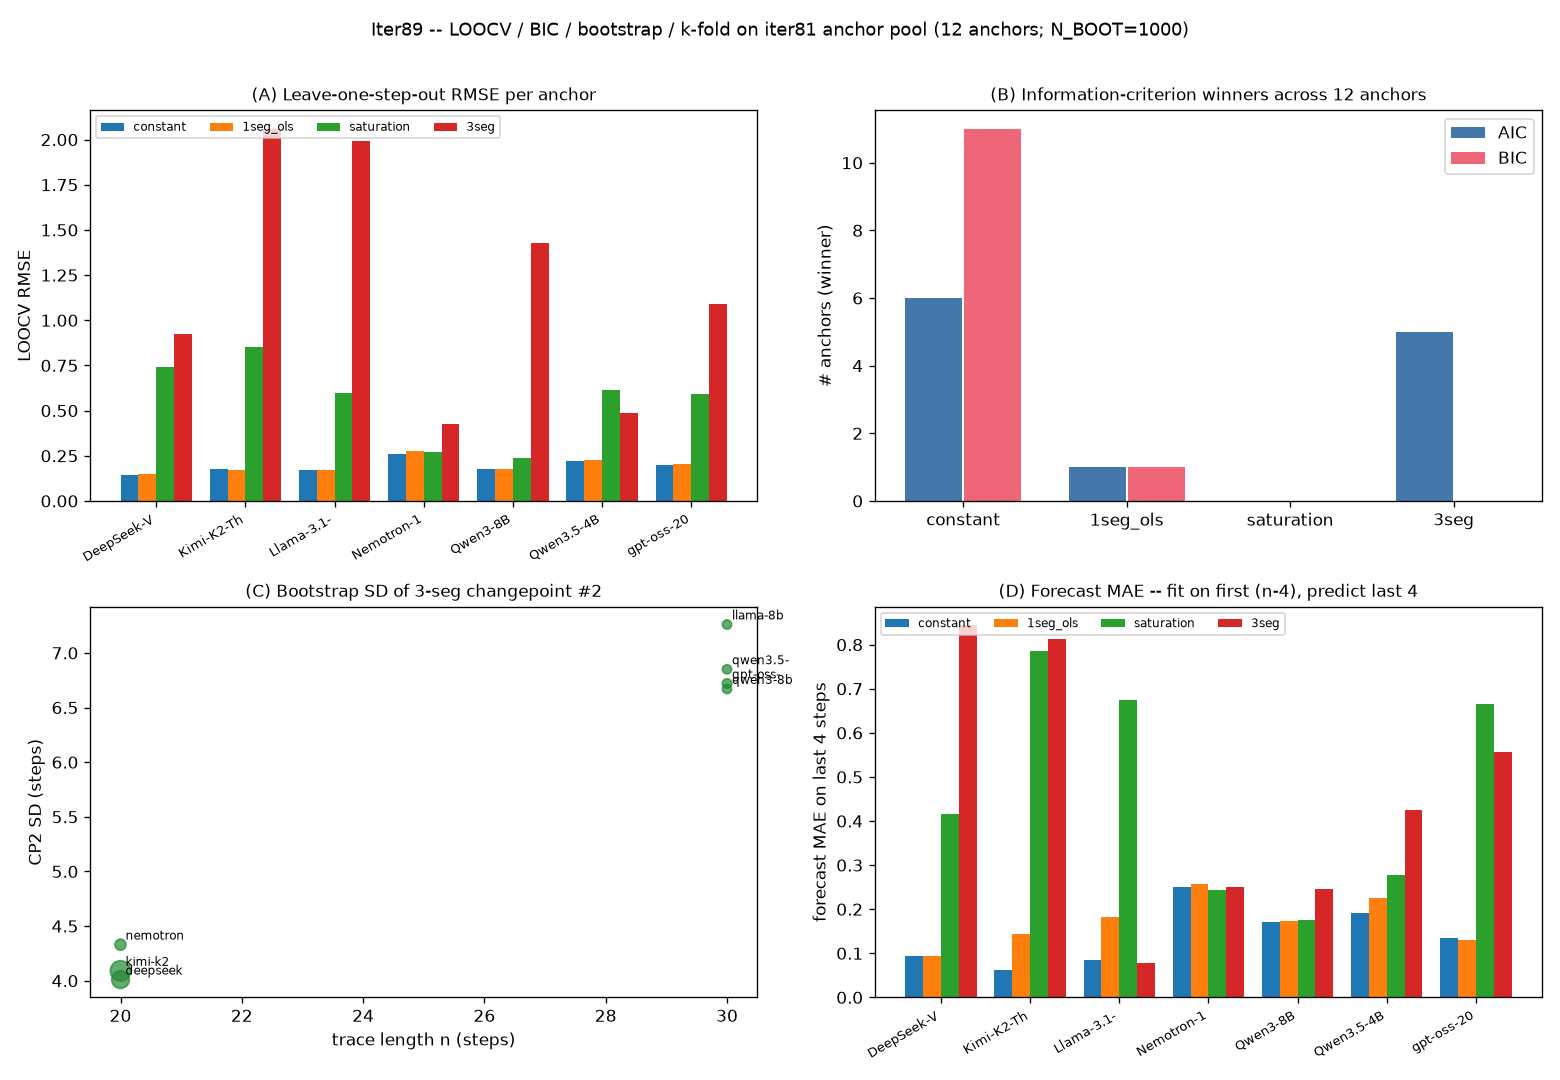
\includegraphics[width=0.92\linewidth]{figures/scaling_law_iter89.png}
\caption{Iter 89 diagnostic battery: (A) leave-one-step-out RMSE per
anchor, grouped by candidate family; (B) AIC vs BIC winner counts
across the 12-anchor iter 81 pool (note: 3-segment drops from 5 to 0
winners); (C) bootstrap SD of the second 3-segment change-point (CP2)
vs trace length; (D) forecast MAE on the last 4 steps when trained on
the first $n-4$.  Constant-mean wins (A), (B), (D); only (C) is a
descriptive plot that confirms the qualitative instability of 3-segment
changepoints under bootstrap.}
\label{fig:scaling-iter89}
\end{figure}

\begin{table}[htbp]
\centering\small
\begin{tabular}{lrrrrr}
\hline
criterion & constant & 1-seg & saturation & 3-seg & total\\
\hline
AIC (in-sample, 12 anchors) & 6 & 1 & 0 & 5 & 12\\
BIC (in-sample, 12 anchors) & 11 & 1 & 0 & 0 & 12\\
LOOCV RMSE (7 anchors) & 6 & 1 & 0 & 0 & 7\\
k-fold forecast MAE (7 anchors) & 4 & 1 & 1 & 1 & 7\\
bootstrap canon-order rate & -- & -- & -- & 24.8\% & --\\
\hline
\end{tabular}
\caption{Iter 89 winner-summary table.  The 3-segment template is the
\emph{only} family that drops from 5 AIC winners to 0 BIC winners and
to 0 LOOCV winners; the constant-mean baseline dominates or ties on
every out-of-sample criterion.  Saturation remains absent from the
winner set in every row, replicating iter 73's falsification under the
stricter model-selection criteria of this iter.}
\label{tab:scaling-iter89}
\end{table}
